% Options for packages loaded elsewhere
\PassOptionsToPackage{unicode}{hyperref}
\PassOptionsToPackage{hyphens}{url}
%
\documentclass[
]{article}
\usepackage{amsmath,amssymb}
\usepackage{lmodern}
\usepackage{iftex}
\ifPDFTeX
  \usepackage[T1]{fontenc}
  \usepackage[utf8]{inputenc}
  \usepackage{textcomp} % provide euro and other symbols
\else % if luatex or xetex
  \usepackage{unicode-math}
  \defaultfontfeatures{Scale=MatchLowercase}
  \defaultfontfeatures[\rmfamily]{Ligatures=TeX,Scale=1}
\fi
% Use upquote if available, for straight quotes in verbatim environments
\IfFileExists{upquote.sty}{\usepackage{upquote}}{}
\IfFileExists{microtype.sty}{% use microtype if available
  \usepackage[]{microtype}
  \UseMicrotypeSet[protrusion]{basicmath} % disable protrusion for tt fonts
}{}
\makeatletter
\@ifundefined{KOMAClassName}{% if non-KOMA class
  \IfFileExists{parskip.sty}{%
    \usepackage{parskip}
  }{% else
    \setlength{\parindent}{0pt}
    \setlength{\parskip}{6pt plus 2pt minus 1pt}}
}{% if KOMA class
  \KOMAoptions{parskip=half}}
\makeatother
\usepackage{xcolor}
\usepackage[margin=1in]{geometry}
\usepackage{longtable,booktabs,array}
\usepackage{calc} % for calculating minipage widths
% Correct order of tables after \paragraph or \subparagraph
\usepackage{etoolbox}
\makeatletter
\patchcmd\longtable{\par}{\if@noskipsec\mbox{}\fi\par}{}{}
\makeatother
% Allow footnotes in longtable head/foot
\IfFileExists{footnotehyper.sty}{\usepackage{footnotehyper}}{\usepackage{footnote}}
\makesavenoteenv{longtable}
\usepackage{graphicx}
\makeatletter
\def\maxwidth{\ifdim\Gin@nat@width>\linewidth\linewidth\else\Gin@nat@width\fi}
\def\maxheight{\ifdim\Gin@nat@height>\textheight\textheight\else\Gin@nat@height\fi}
\makeatother
% Scale images if necessary, so that they will not overflow the page
% margins by default, and it is still possible to overwrite the defaults
% using explicit options in \includegraphics[width, height, ...]{}
\setkeys{Gin}{width=\maxwidth,height=\maxheight,keepaspectratio}
% Set default figure placement to htbp
\makeatletter
\def\fps@figure{htbp}
\makeatother
\setlength{\emergencystretch}{3em} % prevent overfull lines
\providecommand{\tightlist}{%
  \setlength{\itemsep}{0pt}\setlength{\parskip}{0pt}}
\setcounter{secnumdepth}{5}
\usepackage{booktabs}
\usepackage{longtable}
\usepackage{array}
\usepackage{multirow}
\usepackage{wrapfig}
\usepackage{float}
\usepackage{colortbl}
\usepackage{pdflscape}
\usepackage{tabu}
\usepackage{threeparttable}
\usepackage{threeparttablex}
\usepackage[normalem]{ulem}
\usepackage{makecell}
\usepackage{xcolor}
\ifLuaTeX
  \usepackage{selnolig}  % disable illegal ligatures
\fi
\IfFileExists{bookmark.sty}{\usepackage{bookmark}}{\usepackage{hyperref}}
\IfFileExists{xurl.sty}{\usepackage{xurl}}{} % add URL line breaks if available
\urlstyle{same} % disable monospaced font for URLs
\hypersetup{
  pdftitle={Exploratory Analysis},
  pdfauthor={Vildsvinene},
  hidelinks,
  pdfcreator={LaTeX via pandoc}}

\title{Exploratory Analysis}
\author{Vildsvinene}
\date{2023-02-23}

\begin{document}
\maketitle

\renewcommand*\contentsname{Table of Contents}
{
\setcounter{tocdepth}{2}
\tableofcontents
}
\hypertarget{test-section}{%
\section{Test Section}\label{test-section}}

First we load the data:

\begin{table}[H]

\caption{\label{tab:unnamed-chunk-1}First 7 columns of the raw data table}
\centering
\begin{tabular}[t]{llllllr}
\toprule
\textbf{UniqueID} & \textbf{TrackingRound} & \textbf{Sex} & \textbf{CollarID} & \textbf{UTC\_Date} & \textbf{UTC\_Time} & \textbf{Latitude}\\
\midrule
\cellcolor{gray!6}{1\_11855} & \cellcolor{gray!6}{1} & \cellcolor{gray!6}{Male} & \cellcolor{gray!6}{11855} & \cellcolor{gray!6}{2019-02-04} & \cellcolor{gray!6}{15:01:57} & \cellcolor{gray!6}{56.84636}\\
1\_11855 & 1 & Male & 11855 & 2019-02-04 & 16:01:30 & 56.84553\\
\cellcolor{gray!6}{1\_11855} & \cellcolor{gray!6}{1} & \cellcolor{gray!6}{Male} & \cellcolor{gray!6}{11855} & \cellcolor{gray!6}{2019-02-04} & \cellcolor{gray!6}{17:00:45} & \cellcolor{gray!6}{56.84657}\\
1\_11855 & 1 & Male & 11855 & 2019-02-04 & 18:00:15 & 56.84556\\
\cellcolor{gray!6}{1\_11855} & \cellcolor{gray!6}{1} & \cellcolor{gray!6}{Male} & \cellcolor{gray!6}{11855} & \cellcolor{gray!6}{2019-02-04} & \cellcolor{gray!6}{19:00:45} & \cellcolor{gray!6}{56.85110}\\
\addlinespace
1\_11855 & 1 & Male & 11855 & 2019-02-04 & 20:00:15 & 56.85105\\
\bottomrule
\end{tabular}
\end{table}

\begin{table}[H]

\caption{\label{tab:unnamed-chunk-1}Last 7 columns of the raw data table}
\centering
\begin{tabular}[t]{rrrrlll}
\toprule
\textbf{Longitude} & \textbf{DOP} & \textbf{Sats} & \textbf{Temp} & \textbf{TagTime} & \textbf{DropTime} & \textbf{Timestamp}\\
\midrule
\cellcolor{gray!6}{10.22879} & \cellcolor{gray!6}{5.4} & \cellcolor{gray!6}{4} & \cellcolor{gray!6}{16} & \cellcolor{gray!6}{2019-02-04 14:01:00} & \cellcolor{gray!6}{2019-11-21} & \cellcolor{gray!6}{2019-02-04 15:01:57}\\
10.23964 & 2.8 & 5 & 14 & 2019-02-04 14:01:00 & 2019-11-21 & 2019-02-04 16:01:30\\
\cellcolor{gray!6}{10.24342} & \cellcolor{gray!6}{2.4} & \cellcolor{gray!6}{5} & \cellcolor{gray!6}{10} & \cellcolor{gray!6}{2019-02-04 14:01:00} & \cellcolor{gray!6}{2019-11-21} & \cellcolor{gray!6}{2019-02-04 17:00:45}\\
10.25146 & 4.0 & 4 & 12 & 2019-02-04 14:01:00 & 2019-11-21 & 2019-02-04 18:00:15\\
\cellcolor{gray!6}{10.25866} & \cellcolor{gray!6}{3.0} & \cellcolor{gray!6}{6} & \cellcolor{gray!6}{10} & \cellcolor{gray!6}{2019-02-04 14:01:00} & \cellcolor{gray!6}{2019-11-21} & \cellcolor{gray!6}{2019-02-04 19:00:45}\\
\addlinespace
10.25861 & 2.4 & 5 & 10 & 2019-02-04 14:01:00 & 2019-11-21 & 2019-02-04 20:00:15\\
\bottomrule
\end{tabular}
\end{table}

\hypertarget{data-overview}{%
\subsection{Data overview}\label{data-overview}}

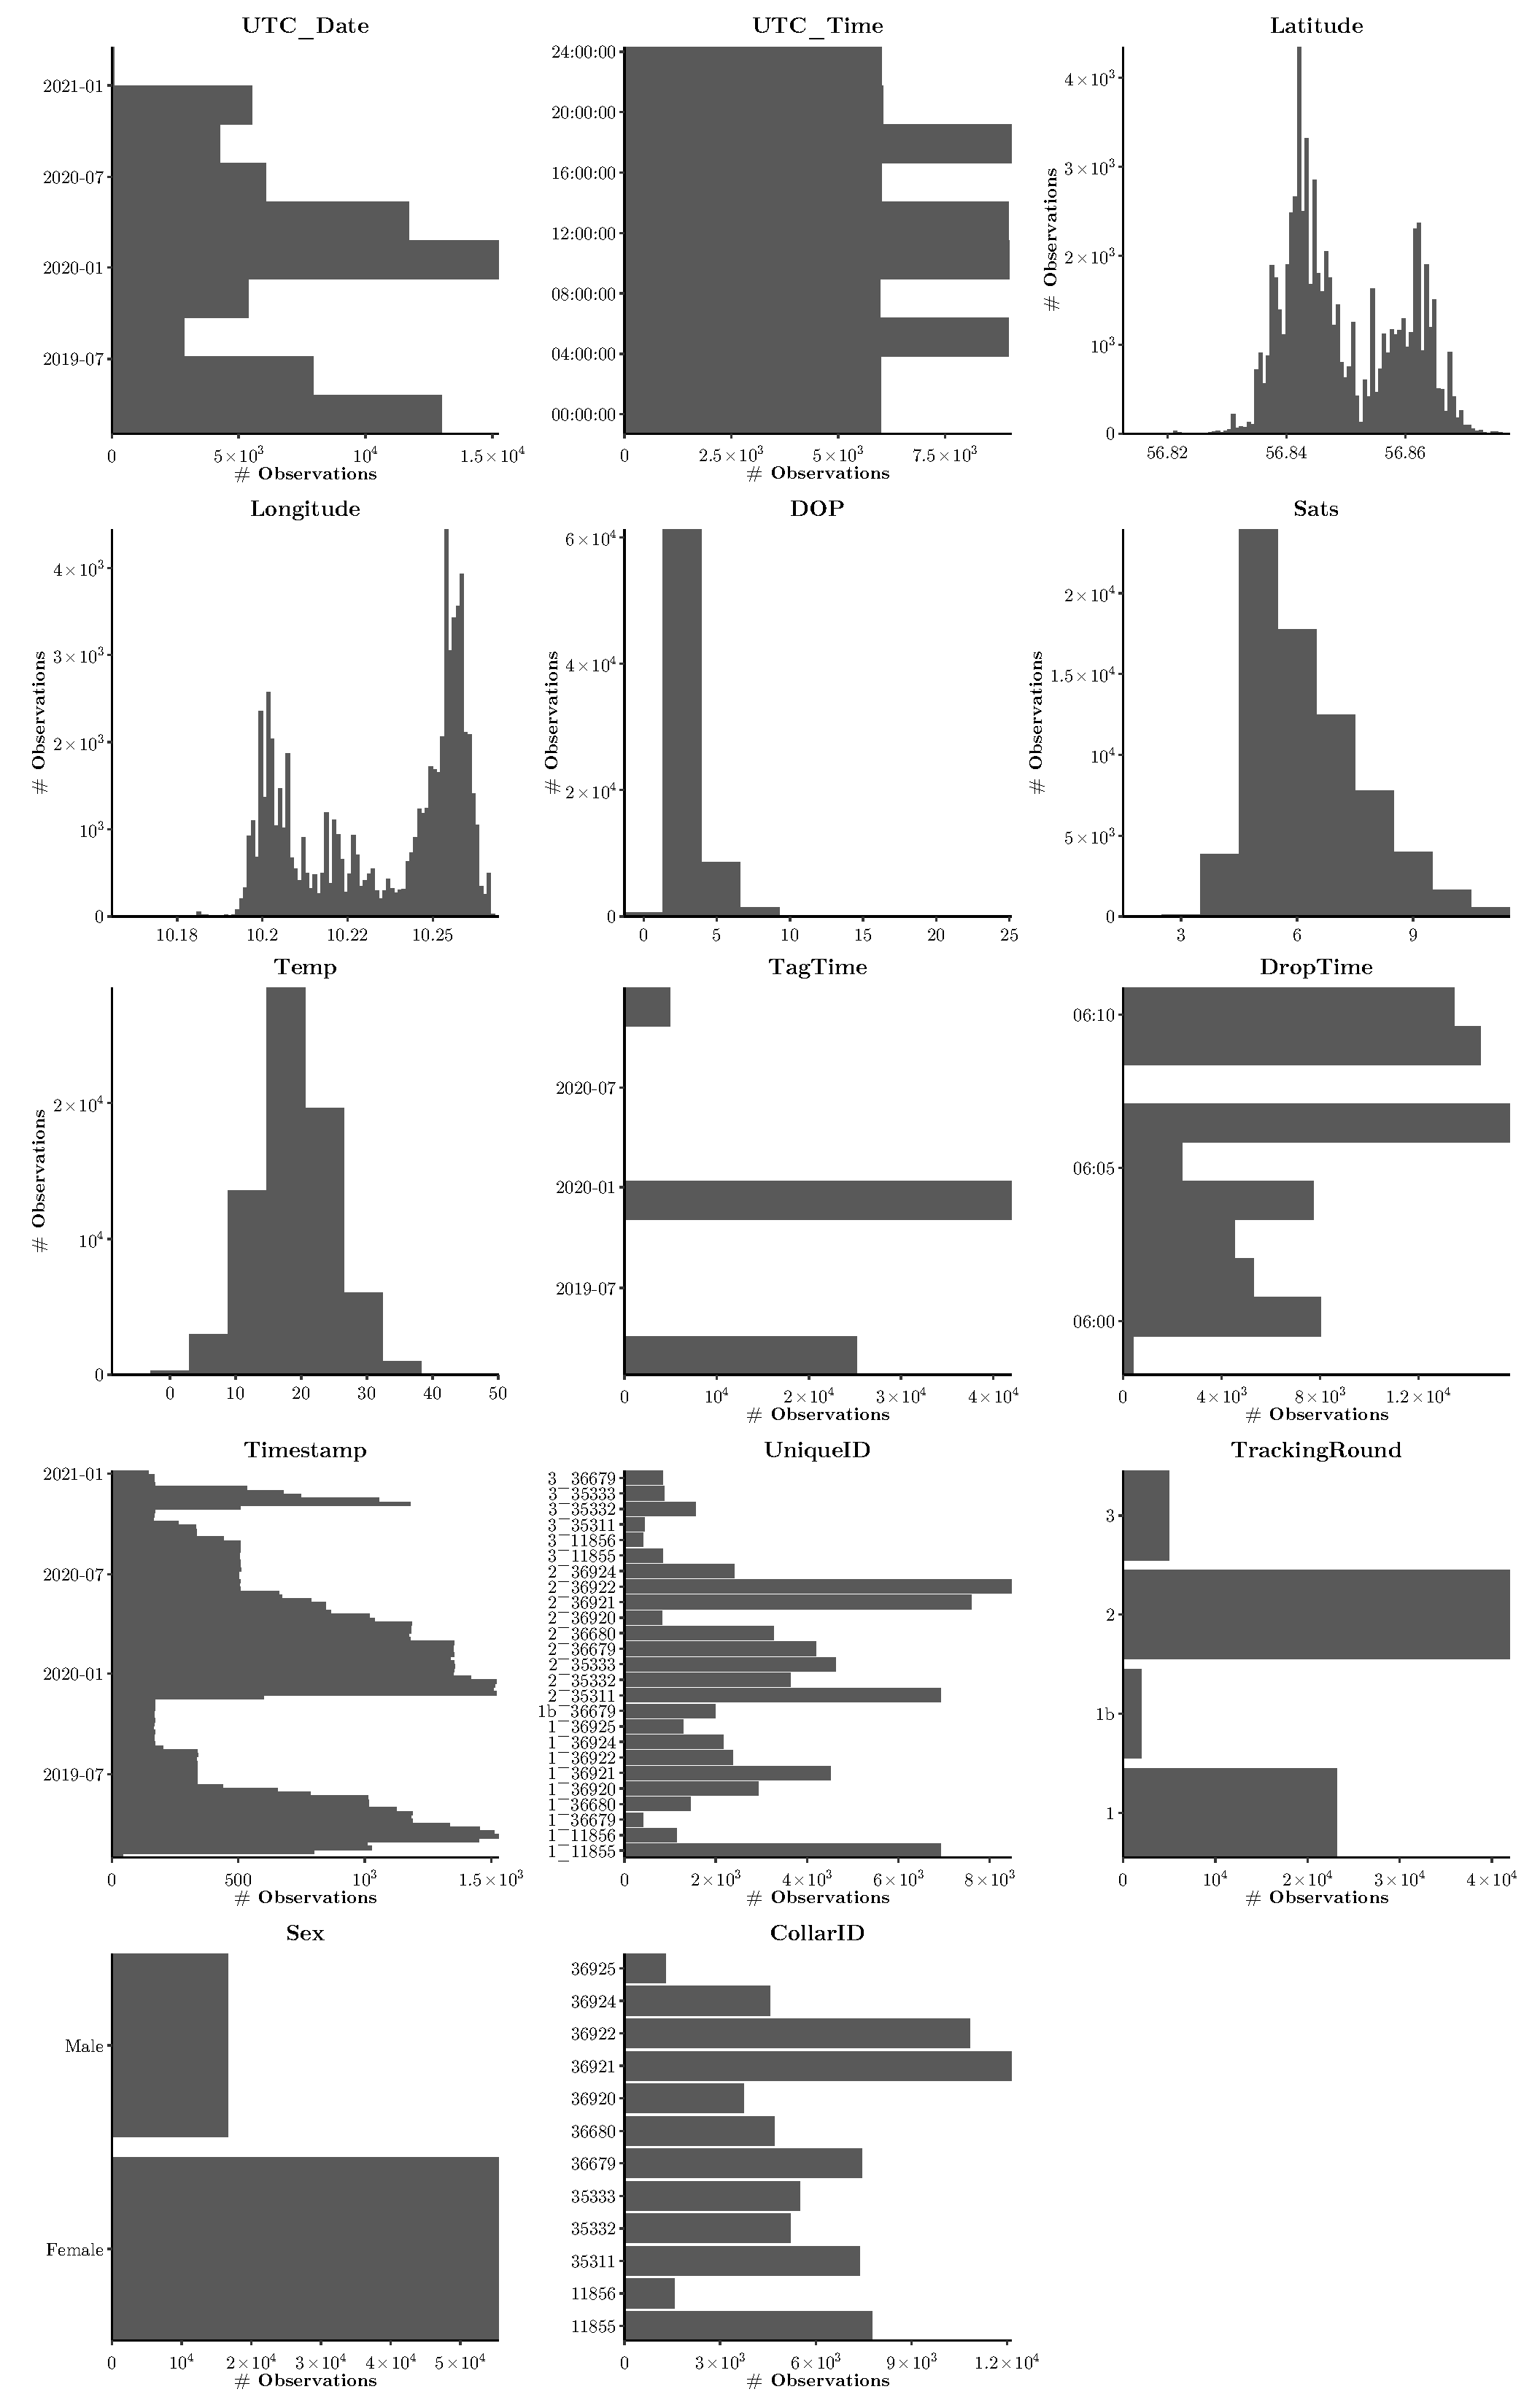
\includegraphics{exploration_files/figure-latex/fig.de-1.pdf}

\end{document}
